%!TeX Program=pTeX-ng(LaTeX)
\special{pdf: mapfile fandol-embeded-scheme1.map}
%\special{pdf: mapfile sim-non-embeded-scheme.map}
%\special{pdf: mapfile sinotype-embeded-scheme.map}
\documentclass[dvipdfmx]{beamer}
\usepackage{hologo}
\usetheme{EastLansing}
\usefonttheme{serif}
\ybaselineshift.5pt
\pdfpagewidth\paperwidth
\pdfpageheight\paperheight
%%%%
\newcommand{\pTeX}{p\kern-.1667em\TeX}
\newcommand{\ptexng}{\pTeX-ng}
\newcommand{\yandy}{Y\kern-.21em{\tiny\&}\kern-.12emY}
%%%%
\begin{document}
\title{\bf \ptexng}
\author{马起园}
\date{2014年11月—12月}
\begin{frame}
\maketitle
\end{frame}
%
\parskip.5zw
\begin{frame}[fragile]
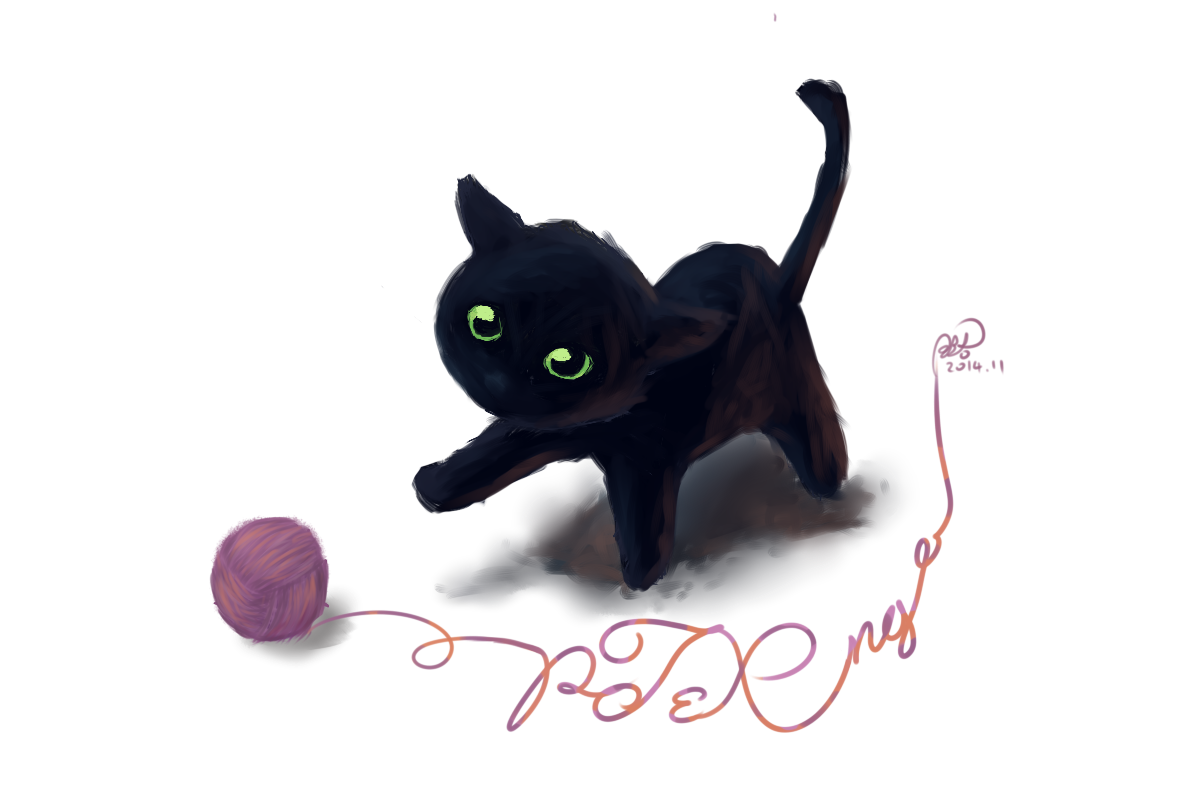
\includegraphics[bb=0 0 864 576, width=\textwidth]{doc-ptex-ng-cat.png}
\end{frame}
\begin{frame}[fragile]
\begin{center}
\ptexng 作者近照$\rightarrow$\lower1zw\hbox{
\includegraphics[bb=0 0 17 17, width=3zw]{doc-ptex-ng-aut.png}}
\end{center}
\end{frame}
%
\begin{frame}[fragile]
\begin{center}
\Huge \ptexng 是一个{\bf 编译器}

\TeX 是一种{\bf 动态语言}
\end{center}
\end{frame}
%
\begin{frame}[fragile]
\frametitle{\bf \ptexng 是什么}
\ptexng 是下一代的\pTeX。在底层引擎上支持汉字处理、禁则处理、汉字和西文间距处理、汉字直排。目前只支持UTF-8编码,覆盖有中日韩三种语言支持。

\pTeX 是日本{\font\t=ascii10 \t ASCII}公司开发的汉字处理引擎。在2008年和2010年经历合并以及收购之后,\pTeX 的实际开发已经停止,已经转向由社区维护。

\ptexng 的开发最早可以追溯到2012年春节假期,最早在Lua\TeX 进行试验性质的修改,在2013年一度中断开发,正式版在今年(2014年)10月份开始发布。由于作者的时间有限,目前只做漏洞修补,下一部分大规模开发要拖到2015年春节。\ptexng 是自由软件,分发遵循GPL第二版许可。
\end{frame}
%
\begin{frame}[fragile]
\frametitle{\bf \ptexng 的开发概要}

\ptexng 的前身是Y\&Y公司的一个用C语言实现的带内存管理的\TeX。早期的源代码是使用{\texttt{web2c}}转换,不具可读性和可扩展性,这部分代码在2014年上半年进行了重写。\ptexng 的源代码建立在这部分代码的基础之上。

\ptexng 的的汉字处理相关代码来源于\pTeX;Unicode编码处理代码来源于u\pTeX。对于\hologo{eTeX}的支持来源于eu\pTeX。

\ptexng 只支持PDF文件输出,相关的代码来源于dvipdfmx,没有任何来自{\textsc{pdf}\TeX}的代码,所以大量primitive不被支持。
\end{frame}
%
\begin{frame}[fragile]
\frametitle{\bf \ptexng 的将来}
\ptexng 在将来会支持OpenType字体、绑定动态语言扩展宏编程。
\begin{enumerate}
\item Lua, Lua 5.2/LuaJIT
\item JavaScript, MuJS/V8/SpiderMonkey
\item Ruby, mruby
\item Scheme, GNU Guile
\end{enumerate}
\end{frame}
%
%\begin{frame}[fragile]
%\frametitle{\bf \ptexng 的equivalent表}
%\def\showeqtb#1#2{{eqtb}[{#1} .. ({#2} - 1)]}
%\begin{enumerate}
%\item \showeqtb{active\_base}{hash\_base},单字符命令
%\item \showeqtb{hash\_base}{glue\_base},非单字符命令(散列表)
%\item \showeqtb{glue\_base}{local\_base},glue参数
%\item \showeqtb{local\_base}{int\_base},临时变量
%\item \showeqtb{int\_base}{dimen\_base},整数变量
%\item eqtb[dimen\_base .. eqtb\_size],长度变量
%\end{enumerate}
%\end{frame}
%
\begin{frame}[fragile]
\frametitle{\bf \ptexng 的catcode}
\begin{center}
\newcommand{\pcc}[1]{\textcolor{red}{#1}}
\begin{tabular}{clcl}
0&escape character&10&space\\
1&beginning of group&11&letter\\
2&end of group&12&other character\\
3&math shift&13&active charactive\\
4&alignment tab&14&comment character\\
5&end of line&15&invalid character\\
6&parameter&\pcc{16}&\pcc{kanji}\\
7&superscript&\pcc{17}&\pcc{hiragana, katakana, alphabet}\\
8&subscript&\pcc{18}&\pcc{cjk symbol codes}\\
9&ignored charcacter&\pcc{19}&\pcc{hangul codes}\\
\end{tabular}
\end{center}
\end{frame}
%
\begin{frame}[fragile]
\frametitle{\bf \ptexng 的primitive}
\begin{itemize}
\item \verb!\jfont!和\verb!\tfont!,这两个和\verb!\font!语义一致。\pTeX 中的TFM有两种,一种是\TeX82定义了的TFM格式;另一种是\pTeX 定义的专门用于重载字符宽度的JFM(后文会专门介绍JFM)。在JFM中,已经定义了对应的文字方向,所以无论使用上述三种那个都不会产生问题。另外,还支持级数和齿数,即Q和H,在大小上为0.25cm,在传统意义上只有前者可用于定义字体大小,后者用来指配其他非字体元素的尺寸。
\item \begin{verbatim}
\font\tenmin=upjisr-h % mincho(KANJI)
\font\sevenmin=upjisr-h at 7pt
\font\fivemin=upjisr-h at 5pt
\end{verbatim}
\end{itemize}
\end{frame}
%
\begin{frame}[fragile]
\frametitle{\bf \ptexng 的primitive}
\begin{itemize}
\item \verb!\kanjiskip!和\verb!\xkanjiskip!,前者会被自动插入到汉字之间,后者会自动插入到非汉字与汉字之间。在\TeX82上,可以使用\texttt{ex}和\texttt{em}。而在\pTeX 中,可以使用\texttt{zw}和\texttt{zh},z表示\textit{zenkaku}(全角,ぜんかく),前者为全角宽度,后者为全角高度。
\item \begin{verbatim}
\kanjiskip=0pt plus .4pt minus .4pt
%\xkanjiskip=2.5pt plus 1pt minus 1pt
\xkanjiskip=.25zw plus 1pt minus 1pt
\end{verbatim}
\end{itemize}
\end{frame}
%
\begin{frame}[fragile]
\frametitle{\bf \ptexng 的primitive}
\begin{itemize}
\item \verb!\tbaselineshift!和\verb!\ybaselineshift!,控制基线的偏移值。前者为直行文本的偏移量,请注意直行的汉字的基线位垂直方向的中心;后者为横行文本的基线偏移量。
\item \begin{verbatim}
\tbaselineshift=3pt
\ybaselineshift=3pt
\end{verbatim}
\item \def\showshift#1{\ybaselineshift#1 \fboxsep.4pt\fbox{林}\hskip\xkanjiskip\fbox{hayasi}\hskip\xkanjiskip\fbox{林}}
\showshift{-1pt}, \showshift{2pt}
\end{itemize}
\end{frame}
%
% \quitvmode
\begin{frame}[fragile]
\frametitle{\bf \ptexng 的primitive}
\begin{itemize}
\item \verb!\ngbanner!,输出默认banner。
\item \ngbanner
\item \verb!\ngostype!,输出当前系统名称。
\item \ngostype
\end{itemize}
\end{frame}
%
\begin{frame}[fragile]
\frametitle{\bf 特别感谢}
\begin{center}
\begin{tabular}{ccccccc}
罗心澄&苏 杰&齐 亮&刘海洋&高 虎&孙 亮&徐腾飞\\
夏晓昊&黄晨成&黄金泽&梁 海&孙 伟&都龙山&王侠兵\\
李国宝&胡玉进&杨海宇&周 浩&曹梦迪&李任之&卢 燚\\
吕文博&翟 羽&钟 毓&肖智博&罗希睿&李 清&张 康\\
王 政&戴唯思&李天池&乔崇智&林 坤&朱文俊&张 麒\\
王昭礼&常金龙&冷俊园&高学远&张伟文&杨笑生&张 潇\\
王 昊&林 科&朱焕杰&李润泽&王 璐&杨林恒&陈甫鸼\\
孙文全&荣健欣&汤进伟&唐俊荣&郝 运&罗晨星&朱 翀\\
何春奇&林懿伦&刘思江&金晨羽&陈 浩&刘中阳&王 冠\\
杨文清&贾泊崴&王 昊&朱 宁&朱佳宁&陈 欣&冷 轩\\
鲁尚文&韩勇杰&&&&&\\
\end{tabular}
\end{center}
\end{frame}
%
\begin{frame}[fragile]
\begin{center}
\ifnum\pdfstrcmp{你}{你}=0
\Huge 休 憩
\fi
\end{center}
\end{frame}
\end{document}
